\documentclass{scrartcl}
\usepackage[mathletters]{ucs}
\usepackage[utf8x]{inputenc}
\usepackage{amssymb}
\usepackage{amsmath}
\usepackage[usenames]{color}
\usepackage{hyperref}
\usepackage{wasysym}
\usepackage{graphicx}
\usepackage[normalem]{ulem}
\usepackage{enumerate}

\usepackage{listings}

\lstset{ %
basicstyle=\footnotesize,       % the size of the fonts that are used for the code
showspaces=false,               % show spaces adding particular underscores
showstringspaces=false,         % underline spaces within strings
showtabs=false,                 % show tabs within strings adding particular underscores
frame=single,                   % adds a frame around the code
tabsize=2,                      % sets default tabsize to 2 spaces
breaklines=true,                % sets automatic line breaking
breakatwhitespace=false,        % sets if automatic breaks should only happen at whitespace
}


\title{Resnet18}
\date{dinsdag 08 december 2020}
\author{}

\begin{document}

\maketitle

		\section{Resnet18}

Created woensdag 18 november 2020



In this page we will describe the results and actions taken to get results out of Resnet18



this paper suggests that this is a good architecture for a quite like problem. where a low amount of data is used.

	\emph{SDD-CNN: Small data-driven convolution neural networks for subtle roller defect inspection}
	


\subsection{Creating first file}



\subsection{TSU\_Resnet18\_1}



failed to load data, did copy files into correct directories and created dataset class



\subsection{TSU\_Resnet18\_2}



Simpeler method to read in data and not be able to change a lot of things;

next time build dataset class self with the same model. 

After that the regression model would be easy



First result of the training.

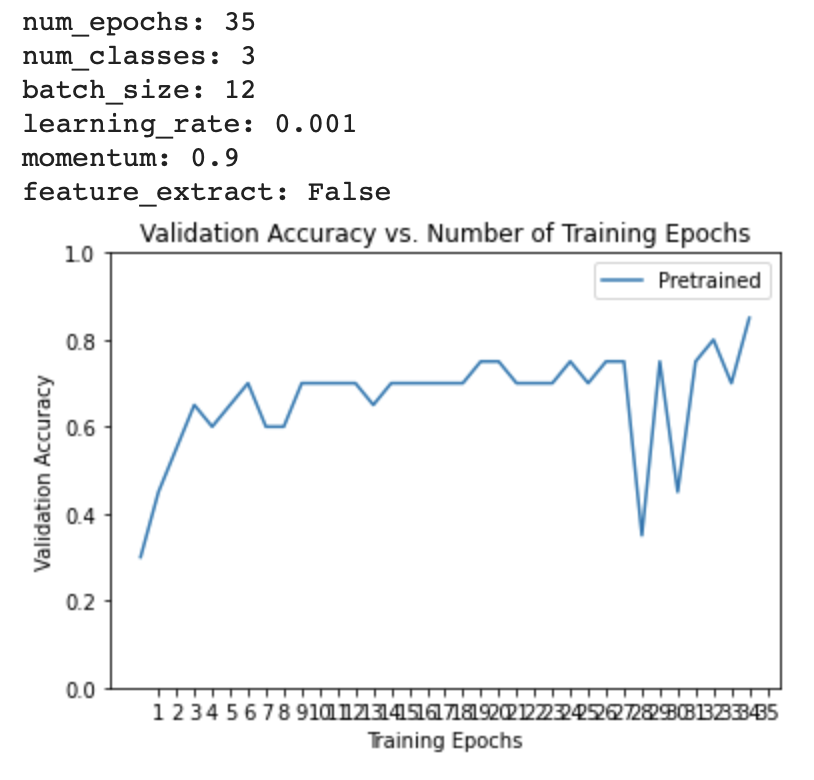
\includegraphics[height=4.166667in, keepaspectratio=true]{./Resnet18/Screenshot 2020-11-18 at 22.58.45.png}

Tweede test met een aanpassing van de learning rate en een foto van de training set naar test set gebracht

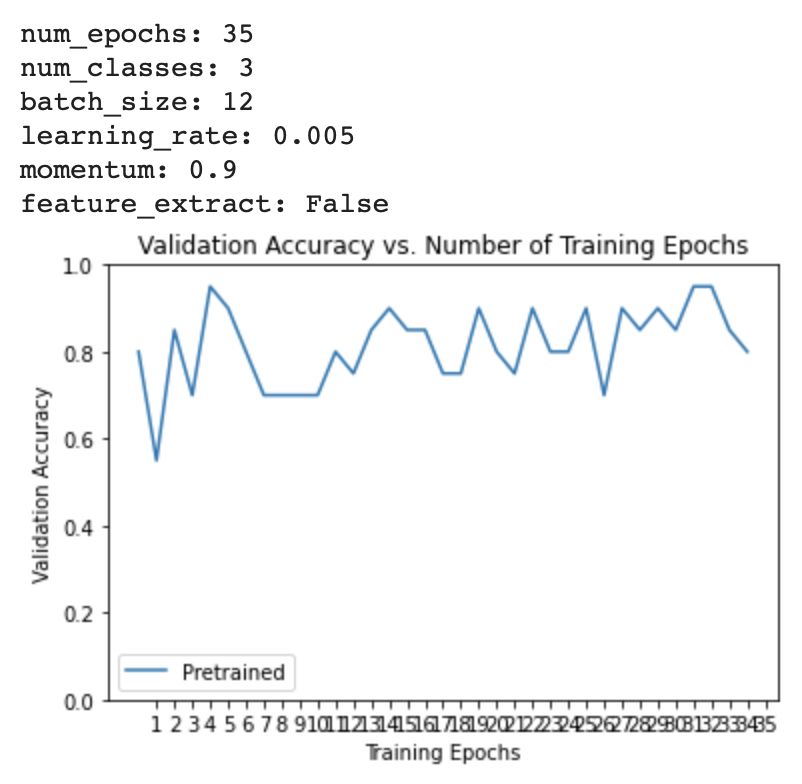
\includegraphics[height=4.166667in, keepaspectratio=true]{./Resnet18/Screenshot 2020-11-18 at 23.13.23.png}



Next time create results file to get nice overview of all results



\end{document}
